\documentclass[a4paper,11pt]{article}
\usepackage{color}
\usepackage{graphicx}
\usepackage{subcaption}
\usepackage{amsmath}
\usepackage{tikz}
\usepackage{listings}
\definecolor{codegreen}{rgb}{0,0.6,0}
\definecolor{codegray}{rgb}{0.5,0.5,0.5}
\definecolor{codepurple}{rgb}{0.58,0,0.82}
\definecolor{backcolour}{rgb}{0.95,0.95,0.92}
 
\lstdefinestyle{mystyle}{
    backgroundcolor=\color{backcolour},   
    commentstyle=\color{codegreen},
    keywordstyle=\color{magenta},
    numberstyle=\tiny\color{codegray},
    stringstyle=\color{codepurple},
    basicstyle=\footnotesize,
    breakatwhitespace=false,         
    breaklines=true,                 
    captionpos=b,                    
    keepspaces=true,                 
    numbers=left,                    
    numbersep=5pt,                  
    showspaces=false,                
    showstringspaces=false,
    showtabs=false,                  
    tabsize=2
}
 
\lstset{style=mystyle}
\usetikzlibrary{automata,positioning}

\graphicspath{ {images/} }
\begin{document}
\title{\color{red}CARNEGIE MELLON UNIVERSITY\\
APPLIED STOCHASTIC PROCESSES  (COURSE 18-751)\\
HOMEWORK 3}
\author{Daniel Marew}
\date{\today}
\clearpage\maketitle

\thispagestyle{empty}
\newpage
I collaborated with :\\
\hspace*{6cm}
Nebyou Yismaw\\
\hspace*{6cm}
Daniel    Nkemelu\\
\hspace*{6cm}
Agatha Niwomugizi
\thispagestyle{empty}
\newpage
\clearpage
\setcounter{page}{1}

\section*{Q1}
\subsection*{(a)}
\subsection*{(b)}
\subsection*{(c)}

\newpage
\section*{Q2}
\subsection*{(a)}
\subsection*{(b)}
\subsection*{(c)}
\newpage

\section*{Q3 \quad Buffers}

\subsection*{(a) for $\lambda = 0.1$, $\mu=0.12$, $BufferSize=10$ and $NumberOf Steps=1000$ we get table\ref{tab:q3} and figure \ref{fig:q3a} }

\begin{table}
\centering
\begin{tabular}{ |c|c|c|c| } 
\hline
 Average Number of packets in Buffer& 3.36  \\
 \hline
 Fraction of time the buffer is empty& 0.33 \\
 \hline
 The fraction of packet Arrivals that are blocked& 0.0040\\
\hline
\end{tabular}
\caption{Question 3b Answer } \label{tab:q3a}
\end{table}•\\\\
\begin{figure}[h]
   \hspace*{-6cm}
    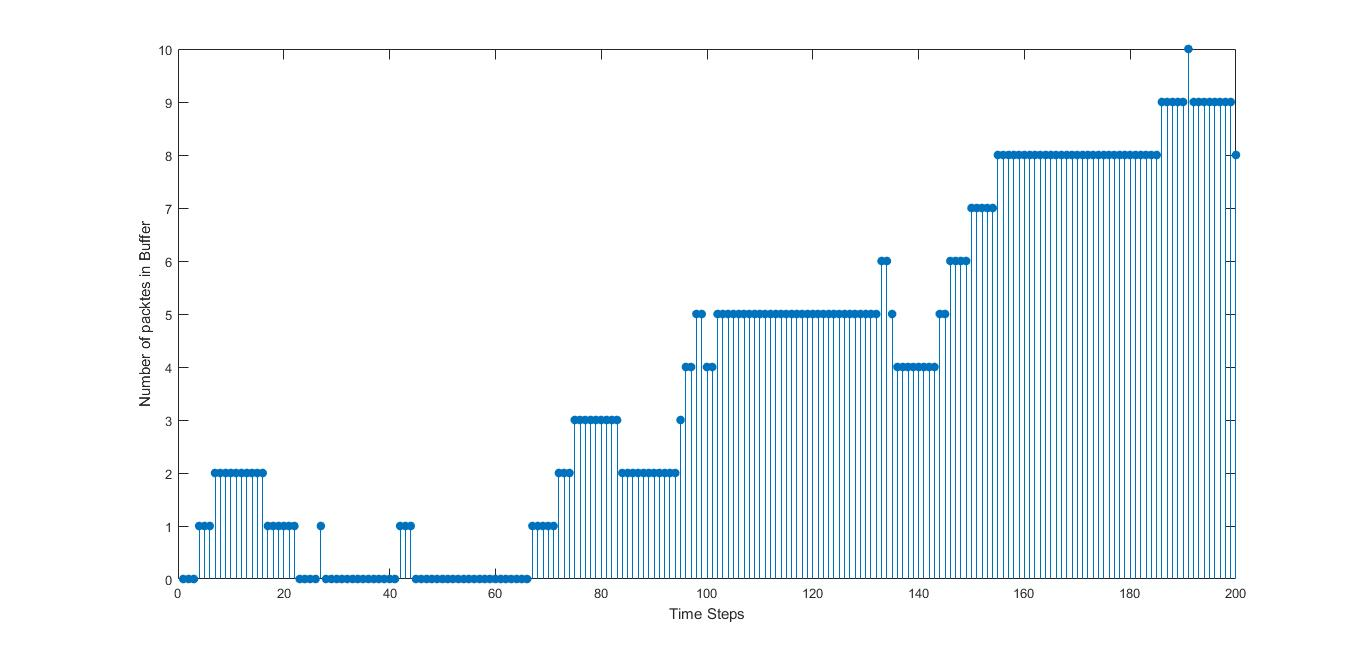
\includegraphics[scale=0.5]{q3_1}
    \caption{Number of packets in the buffer Vs Time steps}\label{fig:q3a}
\end{figure}
\subsection*{(b) for $\lambda = 0.1$, $\mu=0.01$, $BufferSize=10$ and $NumberOf Steps=100$ we get table\ref{tab:q3b} and figure \ref{fig:q3b} }

\begin{table}
\centering

\begin{tabular}{ |c|c|c|c| } 
\hline
 Average Number of packets in Buffer& 6.87  \\
 \hline
 Fraction of time the buffer is empty& 0.03 \\
 \hline
 The fraction of packet Arrivals that are blocked& 0.2100\\
\hline
\end{tabular}
\caption{Question 3 Answer } \label{tab:q3b}
\end{table}•\\\\
\begin{figure}[h]
   \hspace*{-6cm}
    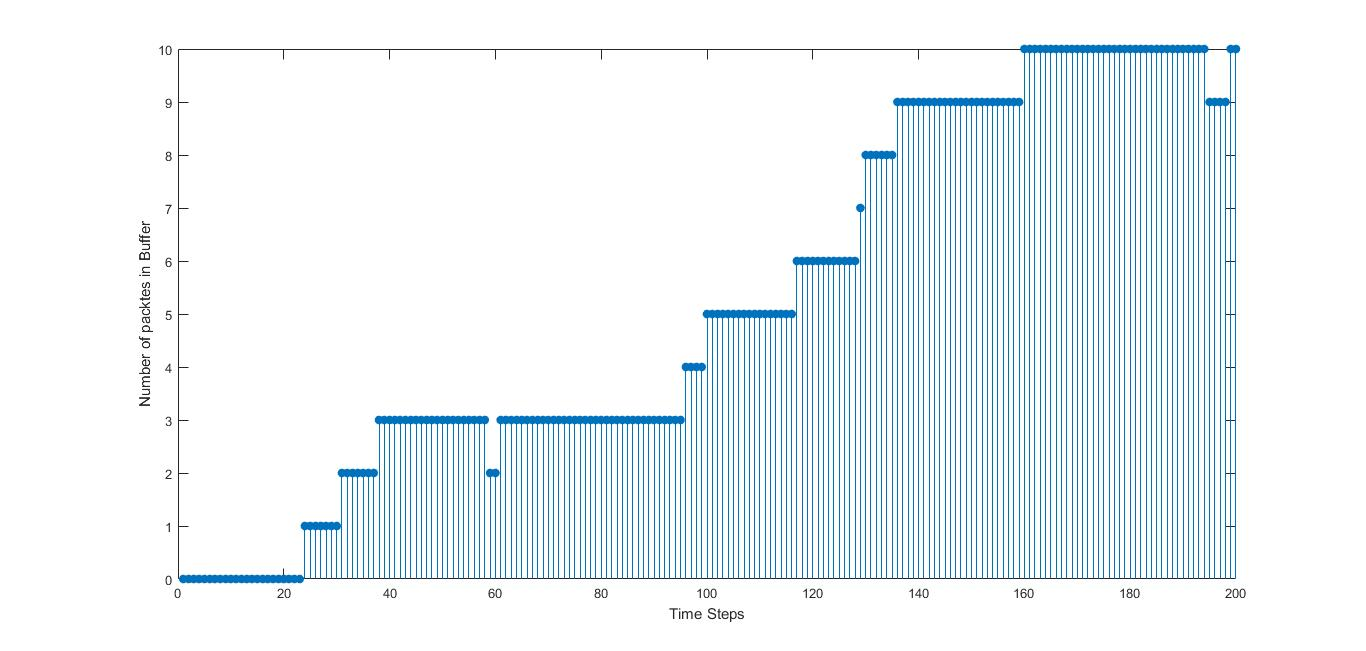
\includegraphics[scale=0.5]{q3_2}
    \caption{Number of packets in the buffer Vs Time steps}\label{fig:q3b}
\end{figure}
\subsection*{(c) Littel Law}
Little Law is given by the following formula \cite{text}\\
\begin{equation}
L = \lambda T
\end{equation}•\\
Where $L$ is the average backlog(the average number of packets in the buffer) , $T$ the delay in the system and $\lambda$ is the average arrival rate.\\\\
hence to get the average delay in the system,
\begin{equation}
T = \frac{L}{\lambda}
\end{equation}•\\
for (a) \\ $$T = \frac{L}{\lambda}=\frac{3.36}{0.1}=33.6$$
for (b) \\ $$T = \frac{L}{\lambda}=\frac{6.87}{0.1}=68.7$$
\newpage

\begin{appendix}
\section*{Code Appendix}
\subsection*{3. a}\label{q3code}
\lstinputlisting[language=Octave]{get_stochastic_matrix.m}  
\lstinputlisting[language=Octave]{q3.m}  
\lstinputlisting[language=Octave]{simMC.m}  
\lstinputlisting[language=Octave]{discrete.m}  
\end{appendix}•
\begin{thebibliography}{9}


\bibitem{text} 
Jean Walrand. 
\textit{Probability in Electrical Engineering and Computer science}. 
Jean Walrand, 2014.

\end{thebibliography}
\end{document}